%%%%%%%%%%%%%%%%%%%%%%%%%%%%%%%%%%%%%%%%%
% Thesis and Articles Template
%
% Author Cosimo Damiano Scarcella
% Date -
%
%%%%%%%%%%%%%%%%%%%%%%%%%%%%%%%%%%%%%%%%%

%----------------------------------------------------------------------------------------
%	PACKAGES
%----------------------------------------------------------------------------------------

\documentclass[12pt,a4paper]{book}
%\documentclass[12pt,a4paper, twocolumn, twoside]{article}
%\documentclass[12pt,a4paper, openright, twocolumn, twoside]{report}
\usepackage[utf8]{inputenc}
\usepackage[italian]{babel}
\usepackage[toc,page]{appendix}
\usepackage{blindtext}% dummy text
\usepackage{amsmath}
\usepackage{amsfonts}
\usepackage{amssymb}
\usepackage{hyperref}
\usepackage{graphicx}
\usepackage{wrapfig}
\usepackage{float}
\usepackage{caption}
\usepackage{subcaption}
\usepackage{listings}
\usepackage[xcdraw,usenames,dvipsnames,svgnames,table]{xcolor}
\usepackage{booktabs}
\usepackage{indentfirst}
\usepackage{pdfpages}
\usepackage{fancyhdr}
\usepackage{calc}
\usepackage{setspace}
\usepackage{fixltx2e}
\usepackage{multicol}
\usepackage[normalem]{ulem}
\usepackage{microtype}     				% microtypography, reduces hyphenation}
\linespread{1.2}
%\pagestyle{fancy}
\frenchspacing
\setlength{\parindent}{0em}

% Color Definition
\definecolor{lightgray}{rgb}{0.83, 0.83, 0.83}
\definecolor{lightblue}{rgb}{0.68, 0.85, 0.9}
\definecolor{lightgreen}{rgb}{0.56, 0.93, 0.56}
\definecolor{lightcyan}{rgb}{0.88, 1.0, 1.0}
\definecolor{lightbrown}{rgb}{0.71, 0.4, 0.11}
\definecolor{gainsboro}{rgb}{0.86, 0.86, 0.86}
\definecolor{beaublue}{rgb}{0.74, 0.83, 0.9}
\definecolor{britishracinggreen}{rgb}{0.0, 0.26, 0.15}
\definecolor{ao(english)}{rgb}{0.0, 0.5, 0.0}
\definecolor{cornellred}{rgb}{0.7, 0.11, 0.11}
\definecolor{periwinkle}{rgb}{0.8, 0.8, 1.0}
\definecolor{platinum}{rgb}{0.9, 0.89, 0.89}

\lstset{%
  backgroundcolor=\color{platinum},		% choose the background color; you must add \usepackage{color} or \usepackage{xcolor}
  basicstyle=\footnotesize,      		% the size of the fonts that are used for the code
  breakatwhitespace=false,         		% sets if automatic breaks should only happen at whitespace
  breaklines=true,                		% sets automatic line breaking
  captionpos=b,                    		% sets the caption-position to bottom
  commentstyle=\color{ao(english)}, 	% comment style
  %deletekeywords={...},            	% if you want to delete keywords from the given language
  %escapeinside={\%*}{*)},          	% if you want to add LaTeX within your code
  extendedchars=true,              		% lets you use non-ASCII characters; for 8-bits encodings only, does not work with UTF-8
  %frame=single,               			% adds a frame around the code
  %frameround=tttt,
  %identifierstyle=\color{black},
  keepspaces=true,                 		% keeps spaces in text, useful for keeping indentation of code (possibly needs columns=flexible)
  keywordstyle=\color{blue},       		% keyword style
  %language=Java,                 		% the language of the code
  %morekeywords={*,...},            	% if you want to add more keywords to the set
  %numbers=left,                   		% where to put the line-numbers; possible values are (none, left, right)
  %numbersep=1pt,                   	% how far the line-numbers are from the code
  numberstyle=\color{purple}, 			% the style that is used for the line-numbers
  rulecolor=\color{black},         		% if not set, the frame-color may be changed on line-breaks within not-black text (e.g. comments (green here))
  showspaces=false,                		% show spaces everywhere adding particular underscores; it overrides 'showstringspaces'
  showstringspaces=false,          		% underline spaces within strings only
  showtabs=false,                  		% show tabs within strings adding particular underscores
  stepnumber=2,                    		% the step between two line-numbers. If it's 1, each line will be numbered
  stringstyle=\color{cornellred},     	% string literal style
  tabsize=2,                       		% sets default tabsize to 2 spaces
  %title=\lstname,                   	% show the filename of files included with \lstinputlisting; also try caption instead of title
  %xleftmargin=\parindent
}
\hypersetup{
    %bookmarks=true,         				% show bookmarks bar?
    unicode=false,          				% non-Latin characters in Acrobat’s bookmarks
    pdftoolbar=true,       					% show Acrobat’s toolbar?
    pdfmenubar=true,        				% show Acrobat’s menu?
    pdffitwindow=false,     				% window fit to page when opened
    pdfstartview={FitH},    				% fits the width of the page to the window
    pdftitle={MyTitle},    					% title
    pdfauthor={Cosimo Damiano Scarcella},   % author
    pdfsubject={MySubject},   				% subject of the document
    pdfcreator={Cosimo Damiano Scarcella},  % creator of the document
    pdfproducer={Cosimo Damiano Scarcella}, % producer of the document
    %pdfkeywords={keyword1} {key2} {key3}, 	% list of keywords
    pdfnewwindow=true,      				% links in new window
    colorlinks=true,       					% false: boxed links; true: colored links
    linkcolor=black,          				% color of internal links (change box color with linkbordercolor)
    citecolor=black,        				% color of links to bibliography
    filecolor=magenta,      				% color of file links
    urlcolor=black           				% color of external links
}
\author{Cosimo Damiano Scarcella}
\title{My Title}
\date{}


%\includepdf{./Chapters/pdf_document.pdf}


\begin{document}
\begin{titlepage}
\begin{center}
{{\Large{\textsc{Text $\cdot$ Text}}}} \rule[0.1cm]{15.8cm}{0.1mm}
\rule[0.5cm]{15.8cm}{0.6mm}
{\small{\bf Text\\
Text }}
\end{center}
\vspace{15mm}
\begin{center}
{\LARGE{\bf My}}\\
\vspace{3mm}
{\LARGE{\bf Title}}\\
\end{center}
\vspace{70mm}
\par
\noindent
\begin{minipage}[t]{0.47\textwidth}
{\large{\bf Text:\\
Text.\\
TEXT}}
\end{minipage}
\hfill
\begin{minipage}[t]{0.47\textwidth}\raggedleft
{\large{\bf Text:\\
TEXT}}
\end{minipage}
\vspace{20mm}
\begin{center}
{\large{\bf Text%inserire il numero della sessione in cui ci si laurea
Text }}%inserire l'anno accademico a cui si è iscritti
\end{center}
\end{titlepage}
\newpage\null\thispagestyle{empty}\newpage %white page

\maketitle
\newpage\null\thispagestyle{empty}\newpage %white page

\frontmatter
\pagenumbering{Roman}
%arabic: Arabic numerals 
%roman: Lowercase roman numerals 
%Roman: Uppercase roman numerals 
%alph: Lowercase letters 
%Alph: Uppercase letters 

\begin{flushright}
\null\vspace{\stretch{1}}
\textit{Dedication}
\vspace{\stretch{2}}\null
\end{flushright}
\newpage
\newpage
\chapter{Summary}

Text Text Text Text Text Text Text Text Text Text Text Text Text Text Text.

\mainmatter
\chapter{Chapter Title}

\section{Text Section}

Text Text Text Text Text Text Text Text Text Text Text Text Text Text Text Text Text.


\section{Figure Section}

\begin{figure}[H]
\begin{center}
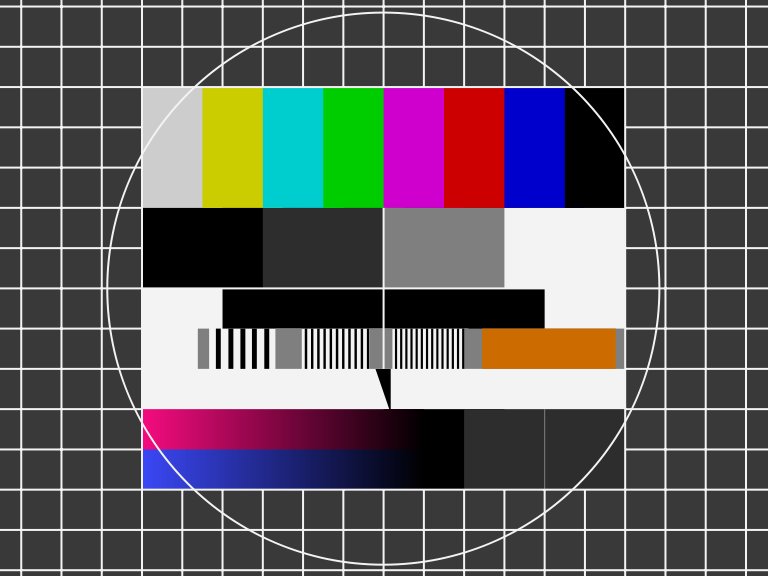
\includegraphics[width=0.8\textwidth]{./Images/test_1.png}
\end{center}
\caption{Figure description}
\end{figure}


\section{Itemize Section}

\begin{itemize}
\item text
\item text
\item text
\item text
\item text
\end{itemize}


\section{Verbatim Section}

\begin{verbatim}
text code
\end{verbatim}


\section{Lstlisting Section}

\begin{lstlisting}[language=bash, frame=single]
text code
\end{lstlisting}


\section{Cite Section}

text \cite{name1}.


\section{Two Figure Comparison Section}

\begin{figure}[H]
        \centering
        \begin{subfigure}[b]{0.5\textwidth}
                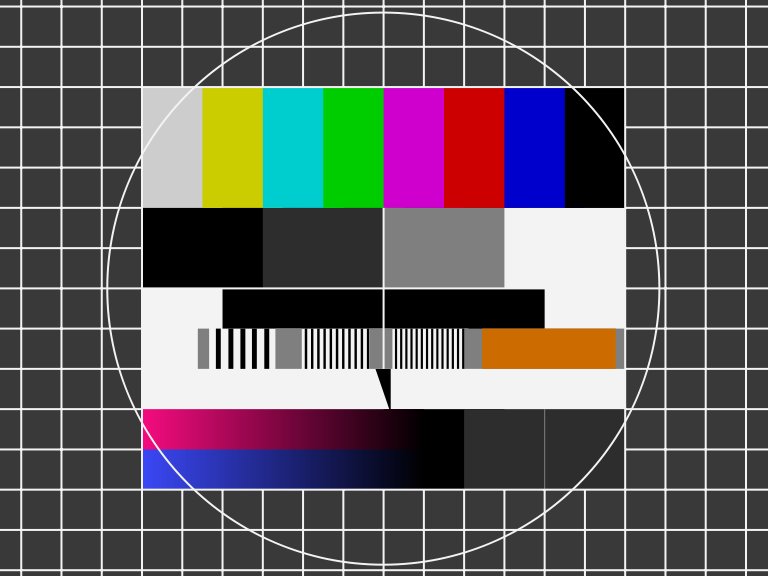
\includegraphics[width=\textwidth]{./Images/test_1.png}
                \caption{\scriptsize Comparison 1}
        \end{subfigure}%
        ~ %add desired spacing between images, e. g. ~, \quad, \qquad, \hfill etc.
          %(or a blank line to force the subfigure onto a new line)
        \begin{subfigure}[b]{0.5\textwidth}
                
\includegraphics[width=\textwidth]{./Images/test_2.png}
                \caption{\scriptsize Comparison 2}
        \end{subfigure}
\end{figure}


\section{Table Section}

\begin{table}[h]                        
\begin{center}		                    % center table
\rowcolors{1}{white}{lightcyan}			% \rowcolors{<starting row>}{<odd color>}{<even color>}
\begin{tabular}[c]{|l|c|r|}             % three columns with vertical lines
										% [b]: bottom
										% [c]: center (default)
										% [t]: top
										% l: left-justified column
										% c: centered column
										% r: right-justified column
										% |: vertical line
										% ||: double vertical line
										% p{'width'}: paragraph column with text vertically aligned at the top
										% m{'width'}: paragraph column with text vertically aligned in the middle (requires array package)
										% b{'width'}: paragraph column with text vertically aligned at the bottom (requires array package)
										% \newline: start a new line within a cell (in a paragraph column)
										% \cline{i-j}: partial horizontal line beginning in column i and ending in column j

\hline                           % inserts a horizontal line
\rowcolor{lightblue}
\textbf{header1} & \multicolumn{2}{c|}{\textbf{header2}}\\ % & separating columns
\cline{2-3}
\hline \hline                           % insert two horizontal lines
text & text & text\\          			% \\ start new row
\hline                                  % insert a horizontal line
text & text & text\\          			% \\ start new row
\hline                                  % insert a horizontal line
text & text & \cellcolor{yellow} text\\
\hline \hline                           % insert two horizontal lines

\end{tabular}
\caption[Table Description]{Table Description}
\end{center}
\end{table}

\appendix 
\chapter{Appendix}

Text Text Text Text Text Text Text Text Text Text Text Text Text Text Text.

\listoffigures
\listoftables 

\frontmatter
\addcontentsline{toc}{chapter}{Bibliography}
\nocite{*}
\bibliographystyle{plain}
\bibliography{./Bibliography/Bibliography}

\tableofcontents
\end{document}